\documentclass[compress,xcolor={dvipsnames}]{beamer}
\usepackage[utf8]{inputenc}
\usepackage[T1]{fontenc}
\usepackage{lmodern}

\usepackage{amsmath}
\usepackage{tikz}
\usetikzlibrary{decorations.pathreplacing,angles,quotes}
\usepackage{graphicx}
\usepackage{listings}
\usepackage{tabularx}

\usetheme{Dresden}
\usecolortheme{spruce}
\usefonttheme[onlymath]{serif}
\beamertemplatenavigationsymbolsempty

%% Listings stuff
\definecolor{color1}{RGB}{244,243,224}
\definecolor{color2}{RGB}{31,174,174}

\definecolor{deepblue}{rgb}{0,0,0.5}
\definecolor{deepred}{rgb}{0.6,0,0}
\definecolor{deepgreen}{rgb}{0,0.5,0}
\definecolor{Keywords}{rgb}{0,0,1}
\definecolor{functions}{rgb}{0.75,0,0.5}
\definecolor{boolean}{rgb}{1,0.4,0}

\lstloadlanguages{C}

\lstset{
    language=C,
    basicstyle=\scriptsize\ttfamily,
    keywordstyle=\ttfamily\color{deepblue},
    commentstyle=\ttfamily\color{deepgreen},
    emphstyle=\color{red},
    showstringspaces=false,
    columns=fullflexible,
    escapechar=£,
    emph={sin,cos,tan,asin,atan,cosh,sinh,exp,log},
    otherkeywords={inline,uint8_t},
    numbers=left,
    mathescape
}
%% End Listings stuff

%% Various macros
\input ./macros.tex


\newenvironment{emphcolor}
               {\usebeamercolor[fg]{title}}
               {\usebeamercolor[fg]{text}}
%% End Macros

\title{Integrating ECLAIR static analysis in IDEs using the Language Server Protocol}

\subtitle{Integrazione dell’analizzatore statico ECLAIR in IDE tramite il Language Server Protocol}

\author{Nicolò Fuccella}

\date{8 settembre 2022}

\begin{document}
%\frame{\titlepage}
\begin{frame}
  \centering

  {\color{green}
  
\includegraphics[height=4em]{logo_unipr_w}
  \vspace{.5em}
  }

  \usebeamercolor[fg]{title}\usebeamerfont{title}\inserttitle

  \usebeamercolor[fg]{subtitle}\usebeamerfont{subtitle}\insertsubtitle

  \vfill
  \usebeamercolor[fg]{author}\usebeamerfont{author}\insertauthor

  \vfill
  \usebeamercolor[fg]{date}\usebeamerfont{date}\insertdate
\end{frame}

\section{Introduction}

\subsection{The Idea}

\begin{frame}
  \frametitle{The Goal}

  \begin{itemize}
   \setlength\itemsep{2em}
    \item
      ECLAIR is a powerful platform for software verification with a strong focus on the development of high-integrity systems, 
      including safety-and security-critical systems.

    \item
      At the moment the check is performed as a separate task, 
      instead we want to integrate the quality assurance from the earlier phases of the development,
      giving feedback to developers about their code correctness while they're writing the code, 
      directly in the IDE.

    \item
      \begin{emphcolor}
        This thesis aims at providing a proof-of-concept of ``immediate feedback software verification'' using ECLAIR.  
      \end{emphcolor}
  \end{itemize}
\end{frame}

\begin{frame}
  \frametitle{The Issues}

  The transition from the traditional way in which static analysis results are consumed to this ``immediate feedback'' modality presents some challenges:

  \begin{itemize}
    \setlength\itemsep{1em}
  
  \item analysis time becomes critical

  \item proliferation of coding environments can lead to a maintenance nightmare

  \item analysis output must be stored in an convenient format in order to be queried

  \end{itemize}
\end{frame}


\subsection{Preliminary Notions}

\begin{frame}
  \frametitle{Preliminary Notions}

  In order to fully grasp the project, it is important to briefly introduce:

  \begin{itemize}
    \setlength\itemsep{1em}
  
  \item program correctness verification

  \item shift-left movement

  \item ECLAIR

  \item the Language Server Protocol

  \end{itemize}
\end{frame}

\begin{frame}
  \frametitle{Program correctness verification}

  \begin{itemize}
    \setlength\itemsep{2em}
  
  \item empirical testing limitations

  \item static analysis pros and cons

  \item static analysis integrations

  \end{itemize}
\end{frame}

\begin{frame}
  \frametitle{Shift-left movement}

  \begin{quote}
    \itshape
    ``Shift-left testing is how I refer to a better way of integrating the quality assurance (QA) and development parts of a software project.  By linking these two functions at lower levels of management, you can expand your testing program while reducing manpower and equipment needs - sometimes by as much as an order of magnitude.'' \footnote{Larry Smith. Shift-left testing. Dr. Dobb's J., sep 2001.}
  \end{quote}
  
  \vspace{1em}

  \begin{quote}
    \itshape
    ``Here is the dilemma in software development: defects are expensive, but eliminating defects is also expensive. However, most defects end up costing more than it would have cost to prevent them.'' \footnote{K. Beck, C. Andres, and E. Gamma. Extreme Programming Explained: Embrace Change., 2004.}
  \end{quote}
\end{frame}

\begin{frame}
  \frametitle{ECLAIR}

  ECLAIR is a powerful platform for software verification. It works on the desktop and on the server to analyze entire projects to:
  \begin{itemize}
    \setlength\itemsep{1em}
    \item automatically detect important classes of software errors
      
    \item validate coding rules, with a particular emphasis on the \begin{emphcolor}MISRA coding standards\end{emphcolor} and others
    
    \item compute software metrics

    \item automatically generate tests
  \end{itemize}
\end{frame}

\begin{frame}
  \frametitle{The Language Server Protocol}
  \large

  \begin{figure}[ht]
    \centering
    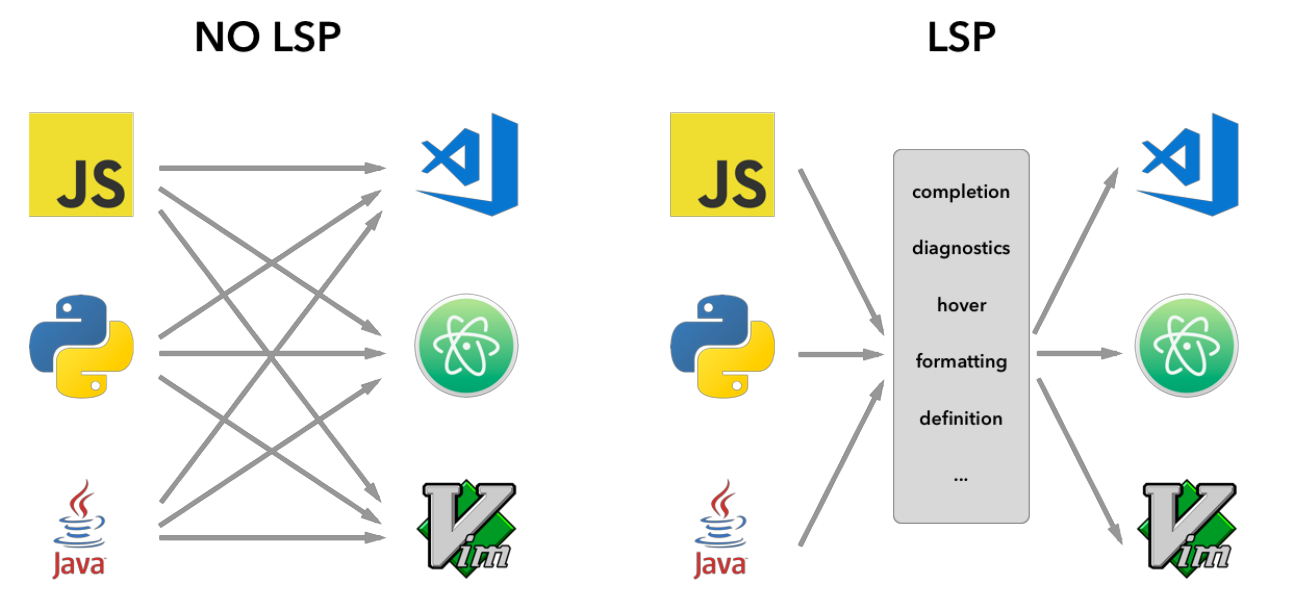
\includegraphics[width=1.0\textwidth]{./language-server-protocol.png}
    \label{fig:one}
  \end{figure}
\end{frame}

\section{Starting point}

\begin{frame}
  \frametitle{Starting point}

  \begin{itemize}
    \setlength\itemsep{2em}
     \item
      The first step was to understand the ECLAIR architecture on top of which we were going to build the prototype.

    \item
      Then we got our hands dirty with a first experiment to fully grasp the potentialities of the Language Server Protocol.
    
    \item
      Finally, we had a clear idea of the issues that needed a more in depth analysis.

  \end{itemize}
\end{frame}

\subsection{The ECLAIR architecture}

\begin{frame}
  \frametitle{The ECLAIR architecture}
  \large

  \begin{figure}[ht]
    \centering
    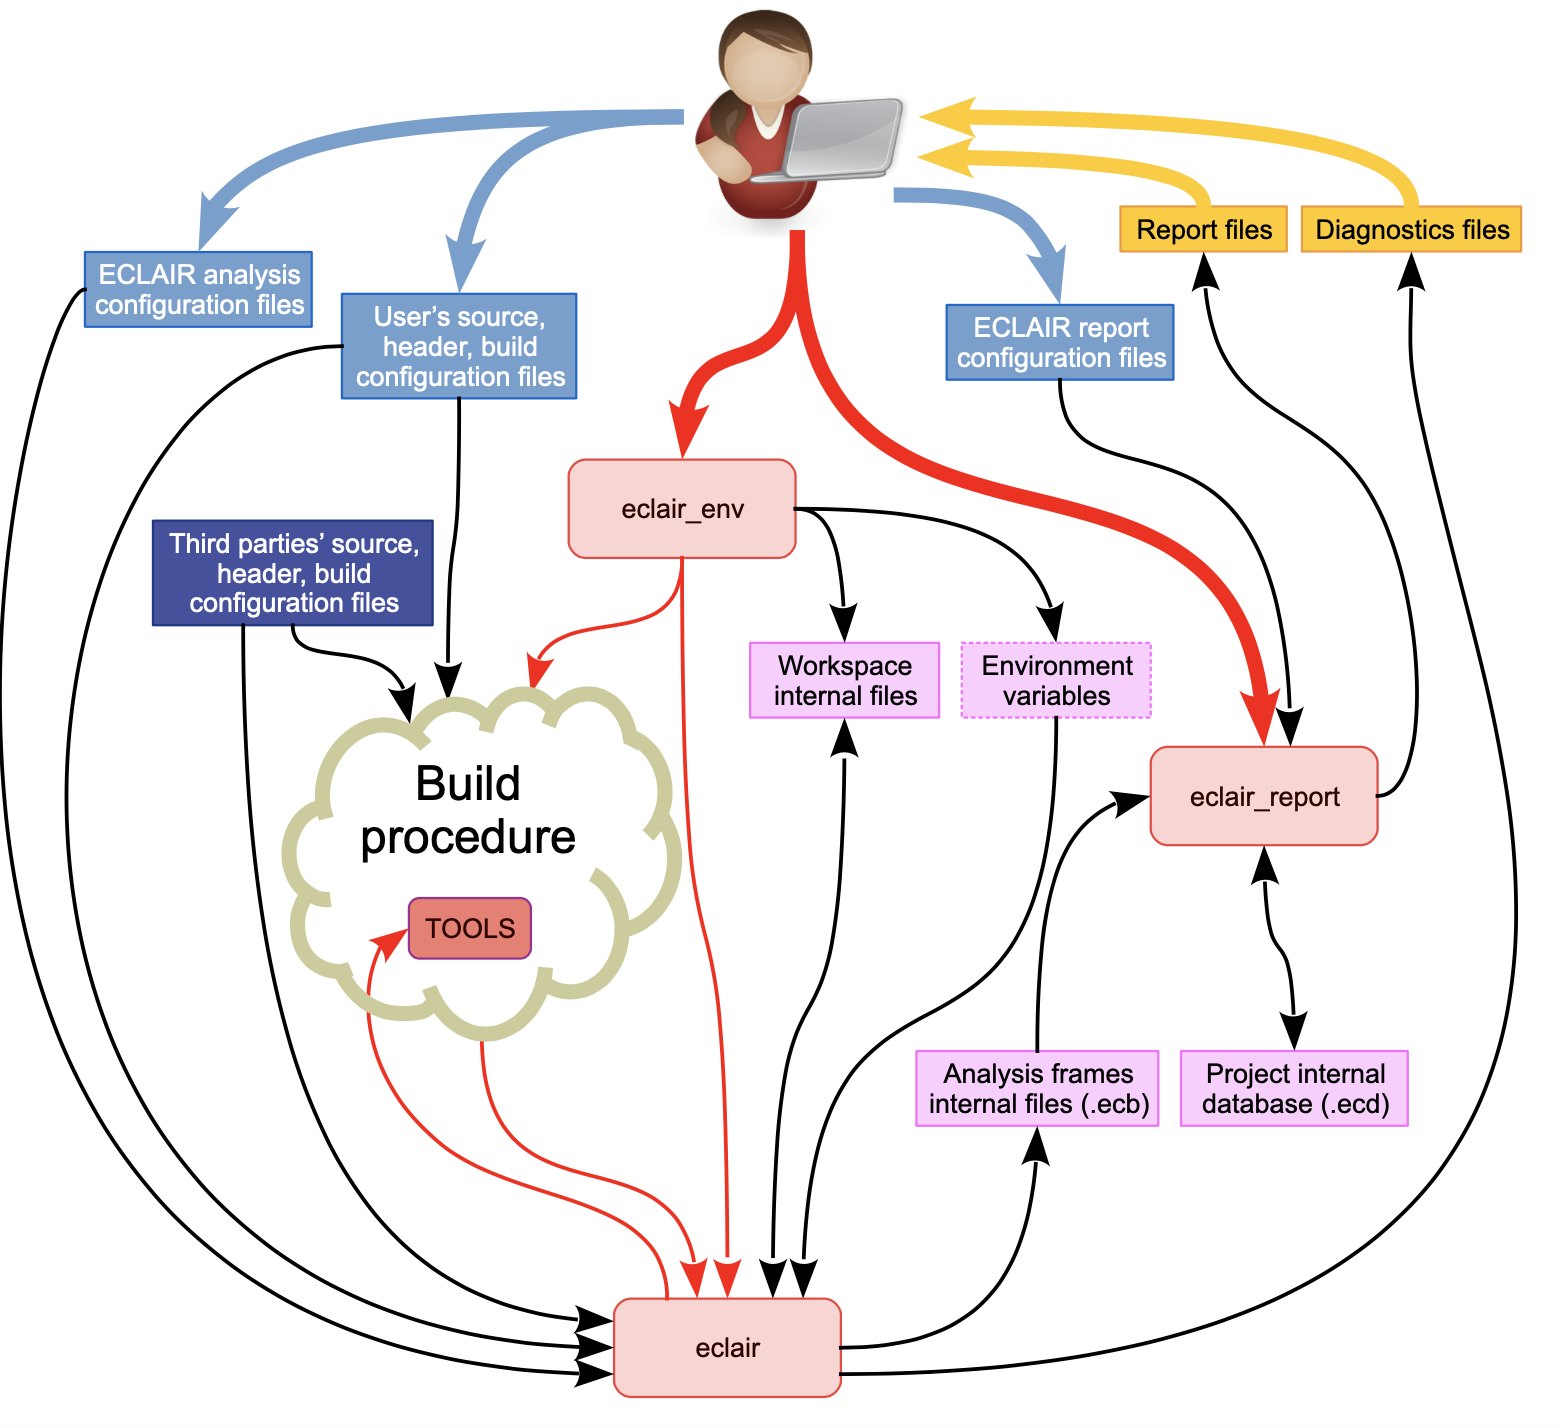
\includegraphics[width=0.6\textwidth]{./ECLAIR_basic_qualifiable_architecture.png}
    \caption{Image copyright by BUGSENG srl, reproduced with permission.}
    \label{fig:one}
  \end{figure}
\end{frame}

\subsection{The first experiment}

\begin{frame}
  \frametitle{The first experiment - Overview}
  \large

  \begin{figure}[ht]
    \centering
    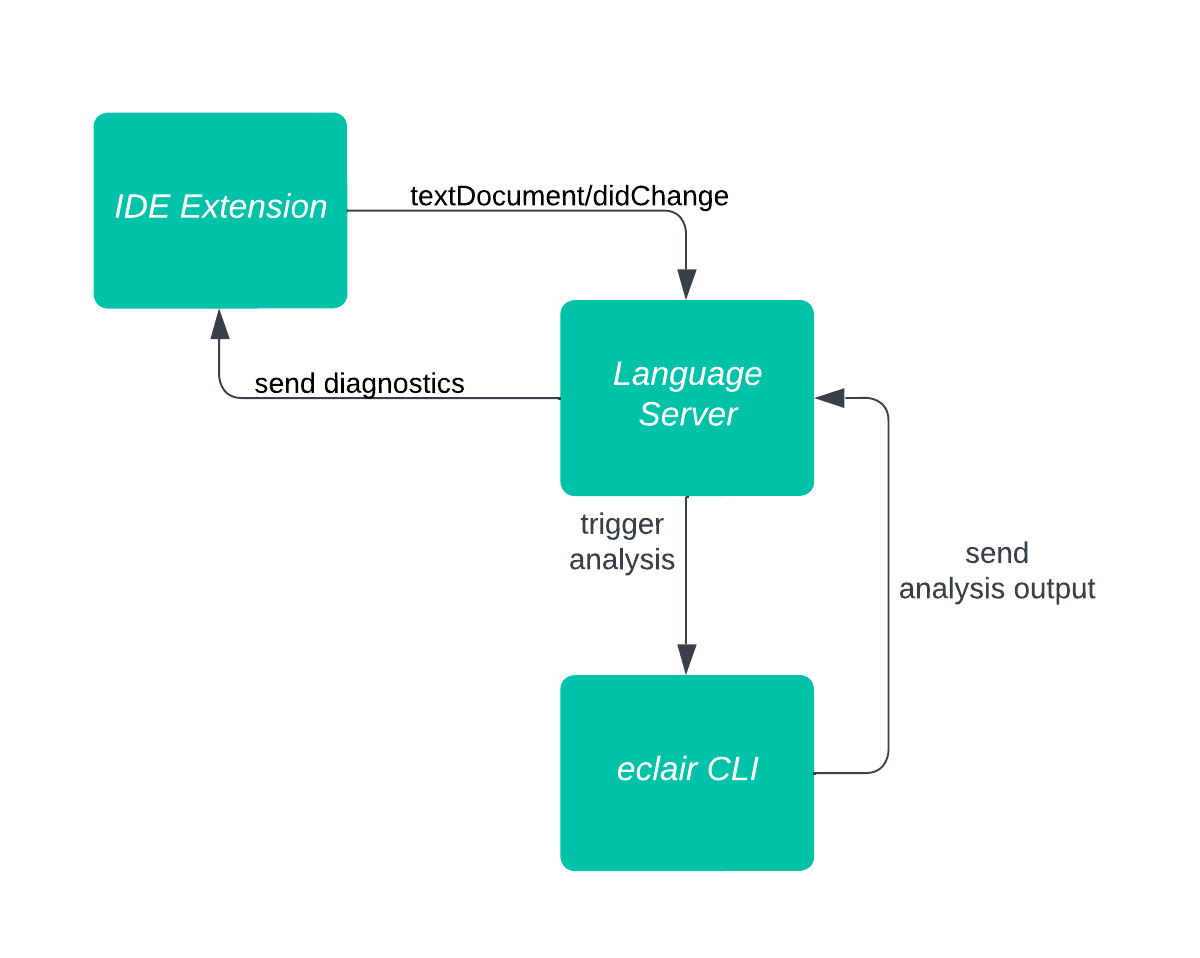
\includegraphics[width=0.8\textwidth]{./the_first_experiment_flow.jpg}
    \label{fig:one}
  \end{figure}
\end{frame}

\begin{frame}
  \frametitle{The first experiment - Lessons learned}
  \large

  \begin{itemize}
    \setlength\itemsep{1em}
  
    \item the analysis cannot be performed whenever the user changes something

    \item violations cannot be returned all at once

    \item the Language Server Protocol reduces dramatically the lines of code needed

    \item some IDE specific features must still be implement from scratch
  \end{itemize}
\end{frame}

\section{The project}

\begin{frame}
  \frametitle{Project architecture}
  \large

  \begin{figure}[ht]
    \centering
    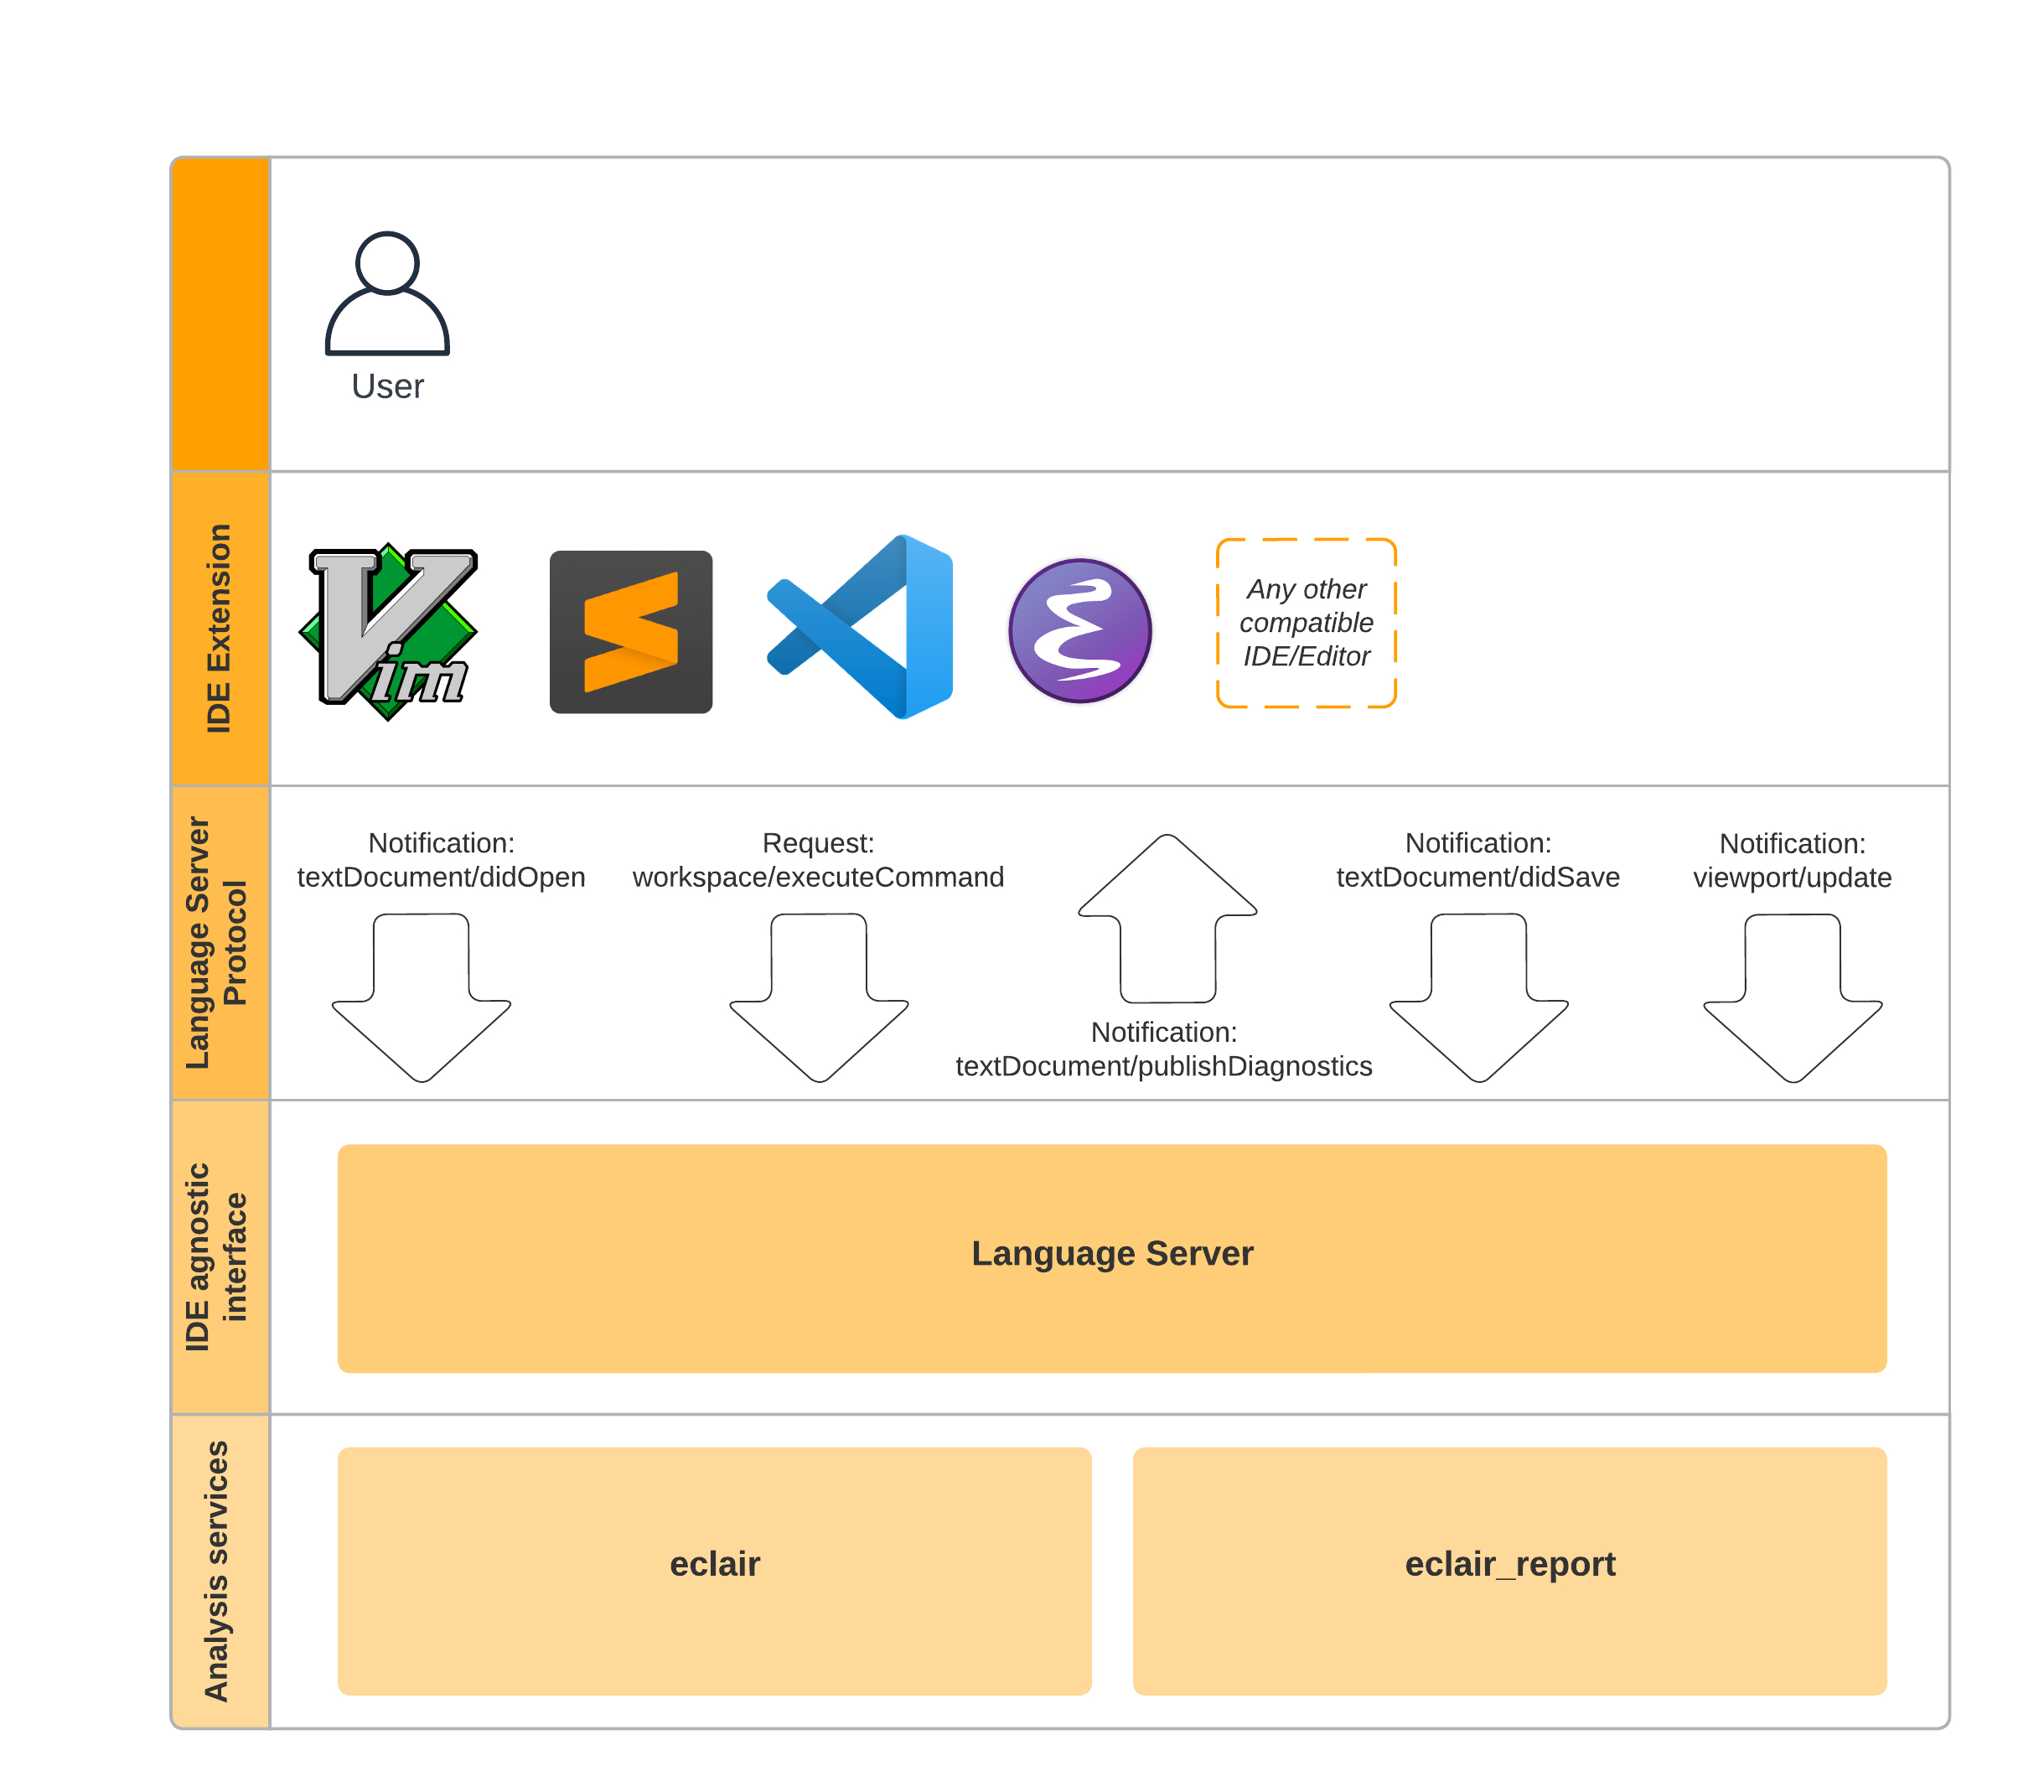
\includegraphics[width=0.7\textwidth]{./project_architecture.jpg}
    \label{fig:one}
  \end{figure}
\end{frame}

\begin{frame}
  \frametitle{Project architecture - Components}
  \large

  Follows an analysis of each component's role:
  \vspace{1em}

  \begin{itemize}
    \setlength\itemsep{2em}
  
    \item \emph{eclair} CLI

    \item \emph{eclair\textunderscore report}

    \item Language Server
  \end{itemize}
\end{frame}

\subsection{Components}

\begin{frame}
  \frametitle{\emph{eclair} CLI}
  \large

  \begin{figure}[ht]
    \centering
    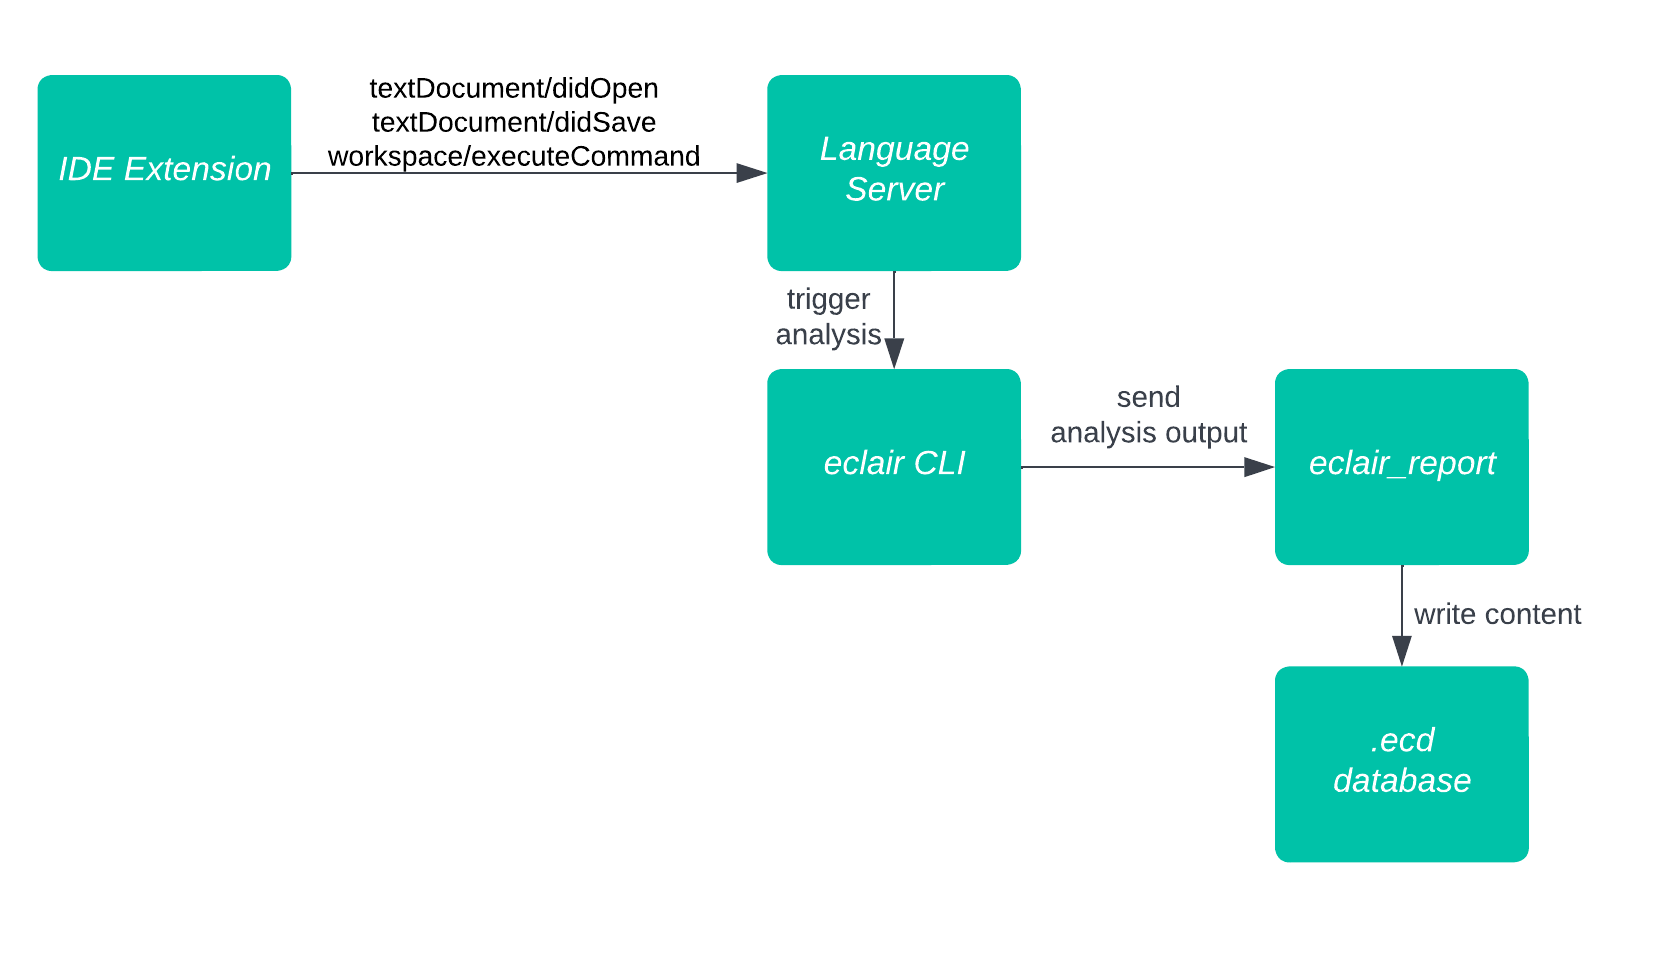
\includegraphics[width=1.0\textwidth]{./eclair_analyzer_flow.png}
    \label{fig:one}
  \end{figure}
\end{frame}

\begin{frame}
  \frametitle{\emph{eclair\textunderscore report}}
  \large

  \begin{figure}[ht]
    \centering
    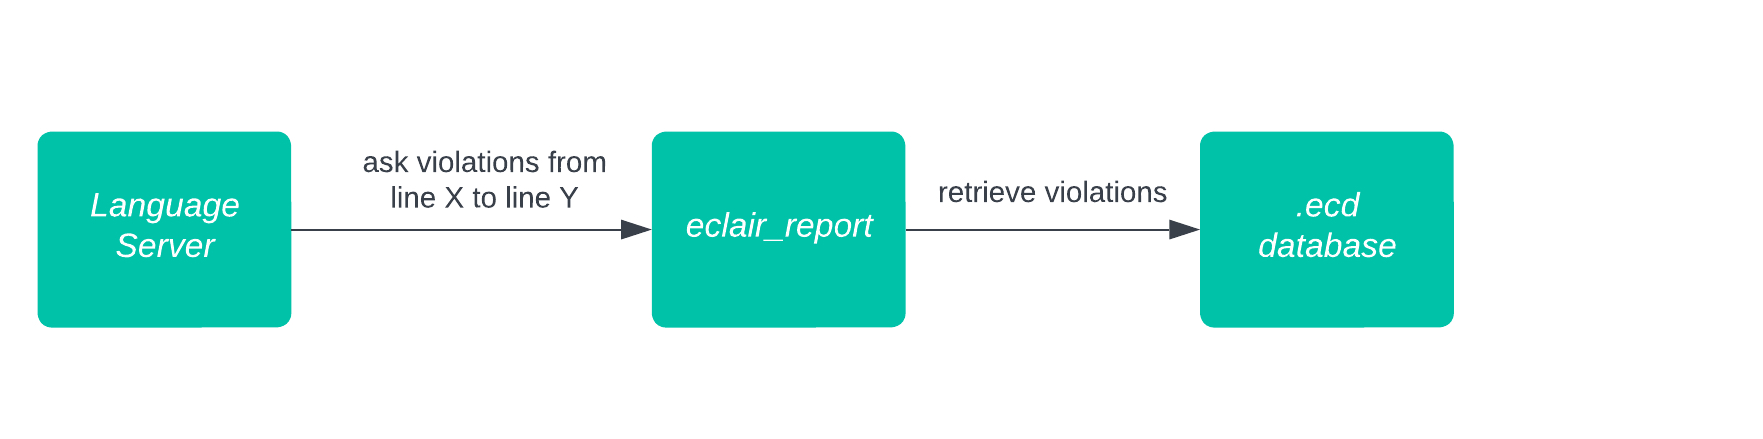
\includegraphics[width=1.0\textwidth]{./eclair_report_flow.jpg}
    \label{fig:one}
  \end{figure}
\end{frame}

\begin{frame}
  \frametitle{Language Server}
  \large

  \begin{figure}[ht]
    \centering
    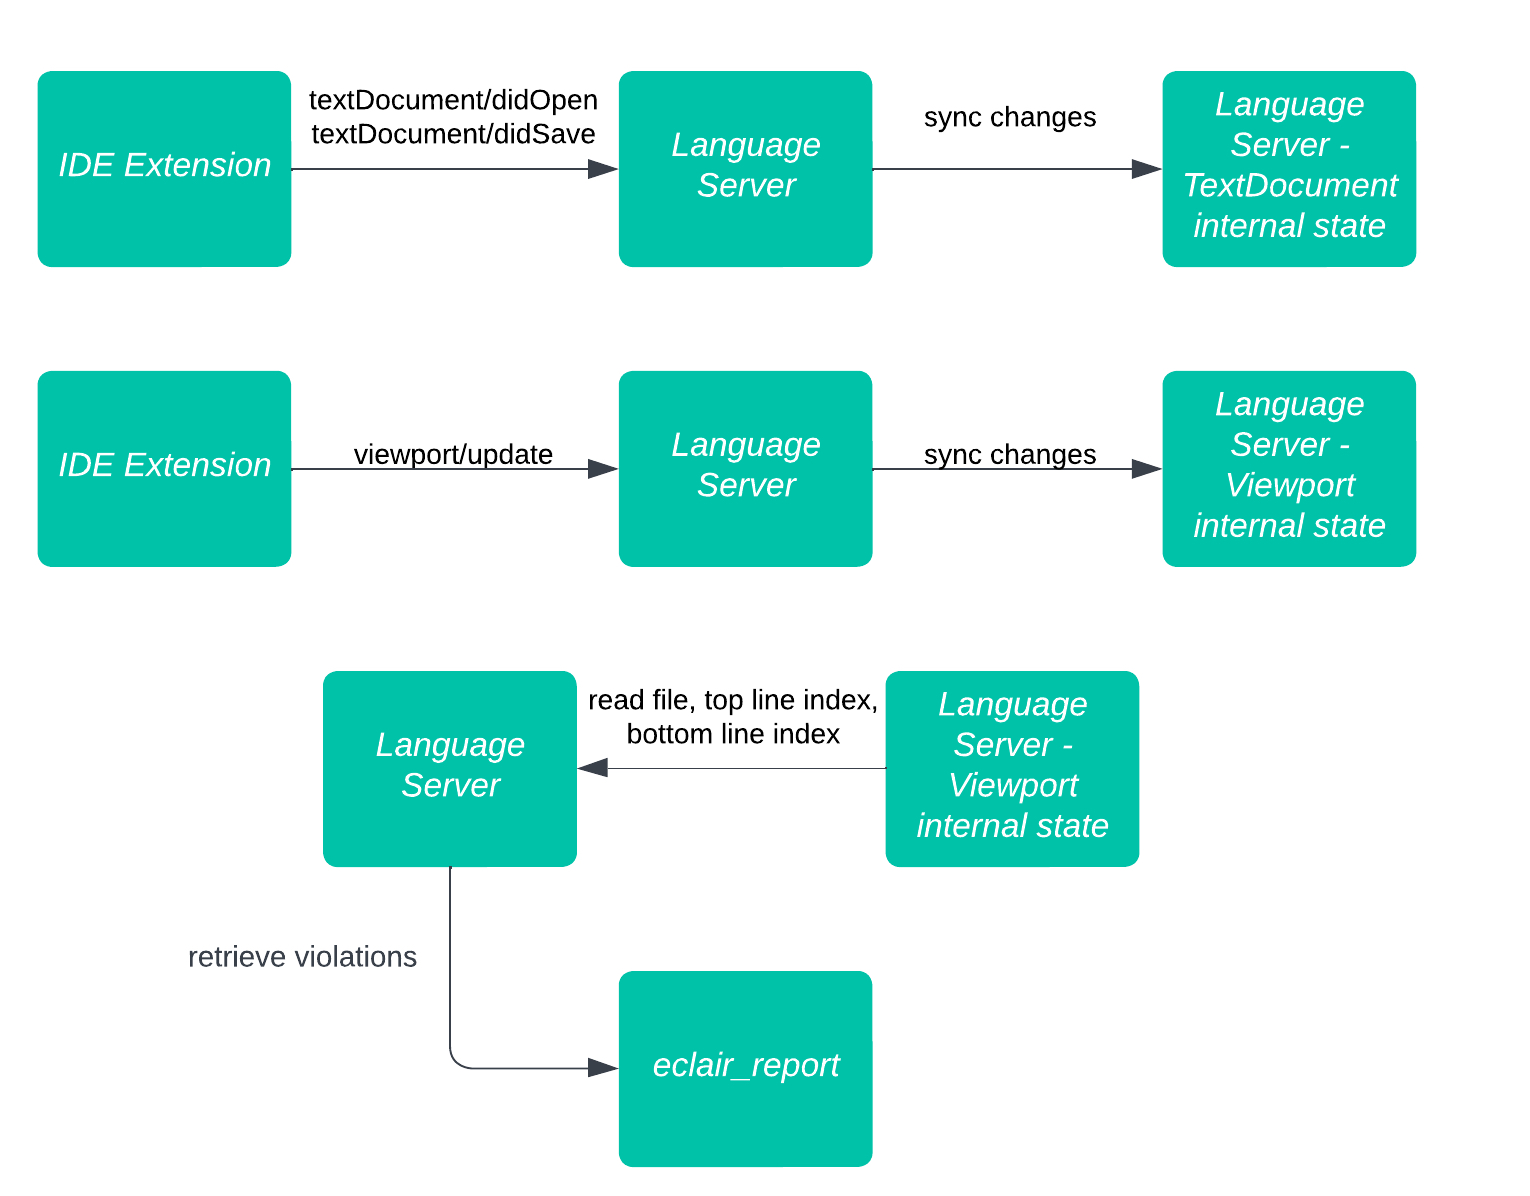
\includegraphics[width=0.8\textwidth]{./language_server_flow.jpg}
    \label{fig:one}
  \end{figure}
\end{frame}

\subsection{The final result}

\begin{frame}
  \frametitle{The final result}
  \large

  \begin{figure}[ht]
    \centering
    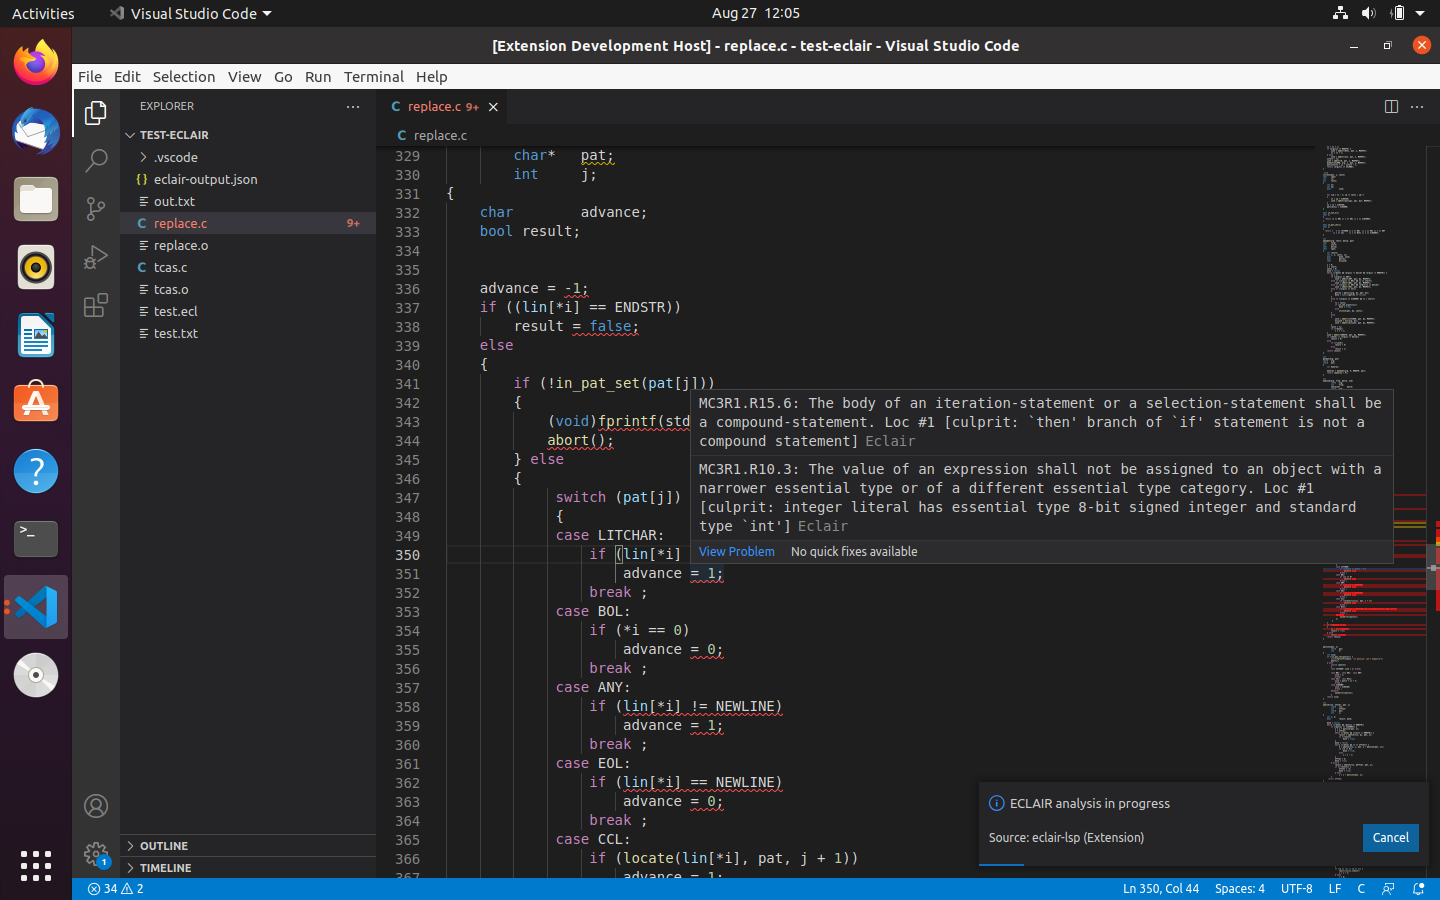
\includegraphics[width=1.0\textwidth]{./vscode_extension_screenshot.jpg}
    \label{fig:one}
  \end{figure}
\end{frame}

\section{The End}

\begin{frame}
  \frametitle{The End}
  \centering

  \begin{emphcolor}
    \Large
    Thank you for your attention.
  \end{emphcolor}
\end{frame}

\end{document}
